\section{Theoretischer Hintergrund}
Dadurch bedingt, das diese Arbeit sich an vielen Konzepten aus der Signaltheorie, Elektrotechnik und Informatik bedient, ist es sinnvoll vorab einige Begriffe und Konzepte zu definieren. Aus diesem Grund, werden im Folgenden das I²C Protokoll, verwendete Software, sowie die genutzte Hardware näher erläutert werden. 

\subsection{Hybrid-Buck-Wandler}
\subsection{I2C}
\begin{flushleft}
I2C steht für Inter-Integrated Circuit und wurde von Philips Semiconductors 1982 entwickelt. Es handelt sich dabei um einen seriellen Datenbus im Master-Slave Stil. Dieses Protokoll setzt auf zwei Leitungen für den Datenaustausch, davon ist ein Kanal explizit für die Daten vorgesehen und der andere Kanal für den Takt. Der Takt beträgt im klassischen 100 KHz oder 400 KHz. 

\begin{figure}
    \centering
    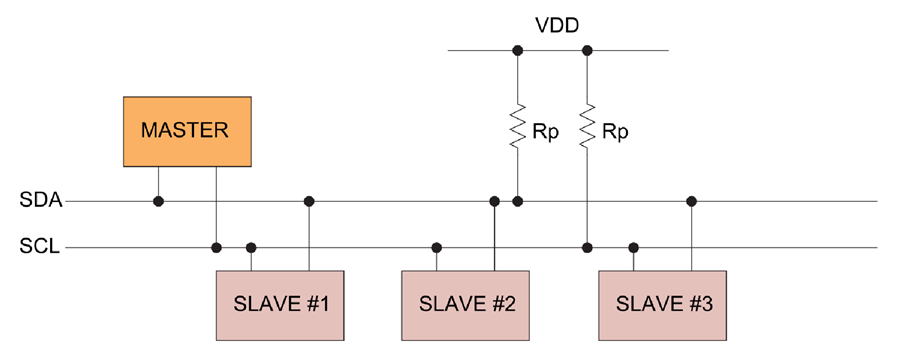
\includegraphics[height= 5cm, width = 10cm]{Pictures/I2C_Bus.png}
    \caption{I2C Bus Beispiel Quelle: https://www.analog.com/en/technical-articles/i2c-primer-what-is-i2c-part-1.html}
\end{figure}

Es ist zu erkennen, dass es eine Master -und mehrere Slave Komponenten gibt. Der Master gibt allen Slaves vor, was sie zu senden haben, und wie schnell sie es tun sollen. Des Weiteren ist zu erkennen, das die beiden Leitungen SDA und SCL an einem Pull-Up Widerstand angeschlossen sind. Dieser dient dazu, die Leitungen, wenn weder Master noch Slave sendet, auf die Versorgungsspannung zu schalten, sodass keine undefinierten Zustände  und die Leitung im unbenutzten Zustand eine logische 1 besitzt. Die Kommunikation erfolgt durch Adressen, so besitzt z. B. jeder Sensor eine I2C Slave Adresse, über die ein Master auf diese zugreifen kann. Das auslesen eines Slaves erfolgt per Registeradressen, so hat beispielsweise ein beliebiger I²C fähiger Sensor ein Register, in dem bestimmte Werte gespeichert sind. In dieser Arbeit handelt es sich bei dem I2C Slave um einen Mikrocontroller auf dem Buck-Wandler. Dieser Slave ist in der Lage Daten zum Strom der Eingangs -und Ausgangsspannung und Temperatur auszugeben. Der Master ist dabei entweder ein PC, welcher per PicKit (I2C auf USB) damit kommuniziert, oder ein Raspberry Pi, welcher direkt per I2C mit dem Netzteil verbunden werden kann.
\end{flushleft}

\subsection{Verwendeten Platformen, Programmiersprachen und Bibliotheken}
\begin{flushleft}

Für die statischen Tests wurde Windows 10 als Platform und C# als Programmiersprache gewählt, da allein diese mit dem PICkit kompatibel sind. 

Da sich herausgestellt hat, dass ein PicKit eine zu geringe Abtastrate ermöglicht, wurde für die dynamischen Tests ein Raspberry Pi 4 (4 GB RAM) mit der Programmiersprache Python für Datenerfassung- und Verarbeitung verwendet.

\end{flushleft}

\subsection{Neuronale Netze}
\begin{flushleft}

Als Klassifizierungsalgorithmus wird ein simples Neuronales Netz verwendet. Neuronale Netze gehören zur Gruppe vom "Supervised Learning" (dt. "Betreutes Lernen"). Das Konzept von diesem Algorithmus ist es, dem Model einen Datensatz und die dazugehörige Lösung zu geben. Ausgehen davon passt das Neuronale Netz seine Parameter an. Dieser Vorgang wird im Folgenden formell erläutert.

Zur durchführung von einigen simplen Testfällen unter Punkt 3.3 ist es notwendig eines der Grundlegenden Konzepte von Machine Learning zu nennen: das Neuronale Netze. Neuronale Netze sind in ihrem Grundgedanken dem Konzept des menschlichen Gehirns nachempfunden jedoch in vielerlei hinsicht anders. In Abb. 2 erkennt man ein Diagram eines Neuronalen netzes. Die Kreise repräsentieren die Neuronen, die Kante stellen Verbindungen unter den Neuronen dar. Es ist zu beachten, das in diesem Model die Neuronen von einer Schicht N vollvermascht mit den Neuronen einer Schicht N+1 sind. Des Weiteren ist zu erkennen, dass der dargestellte Graph drei Schichten (engl. Layers) besitzt. \hl{ Der Input Layer dient dabei als Ausgangspunkt, an dieser Stelle wird in jedes Neuron ein numerischer Wert eingespeist. Alle Werte im Input Layer zusammengenommen ergeben einen Vektor V.}

Abschließend erfolgt eine weitere Matrixmultiplikation des Hidden Layers und seinen Weights, um das Output Layer zu generieren. Das Output Layer gibt, wie der Name schon sagt, die Ausgangswerte der Berechnung. Bei Klassifizierungsaufgabe sind die Werte im Output Layer Warscheinlichkeiten für die jeweiligen, zu klassifizierenden Klassen. Die Anzahl der Neuronen im Output Layer ist gleich der Anzahl der Klassen
\end{flushleft}

Die Formel für Feedforward:  


Die Formel für die Sigmoid Funktion: 

\begin{equation}
\label{Sigmoid}
s(z) = \frac{1}{1+e^{-z}}
\end{equation}

\end{flushleft}
